\documentclass[../main.tex]{subfiles}

\begin{document}


The following is the definition of the residual.
\begin{center}
    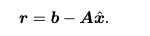
\includegraphics[width=\textwidth,height=\textheight,keepaspectratio]{lec6_resid}
\end{center}

\begin{remark}
    The residual itself does not reveal much. Suppose we calculate $r = b - Ax$. Now solve for $kAx = kb$ and the residual required to solve that is $k$ times as great. This is why we define the relative residual:

    \[
        \frac{\norm{r}}{\norm{A} \cdot \norm{\hat{x}}}
    \]
\end{remark}

We can obtain a bound on the relative forward error required to solve $Ax = b$ in terms of $r$.
\begin{center}
    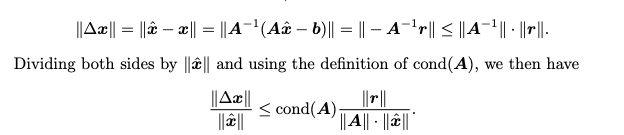
\includegraphics[width=\textwidth,height=\textheight,keepaspectratio]{lec6_residBound}
\end{center}

\begin{remark}
    This bound tells us that if the residual is small and the matrix and well conditioned, then the relative error is low.
\end{remark}

\begin{center}
    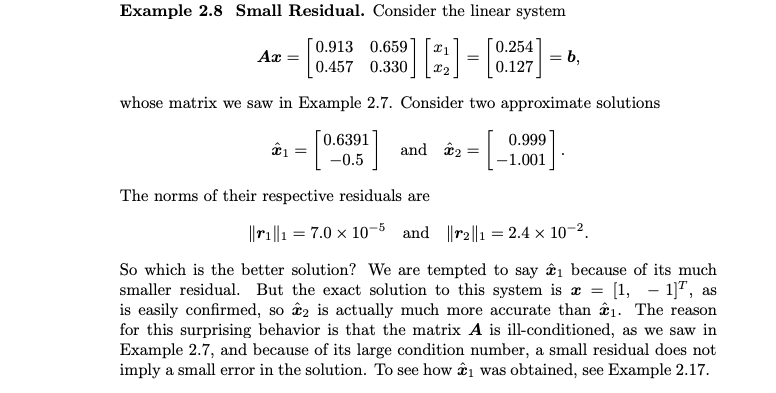
\includegraphics[width=\textwidth,height=\textheight,keepaspectratio]{lec6_residExample}
\end{center}

\begin{center}
    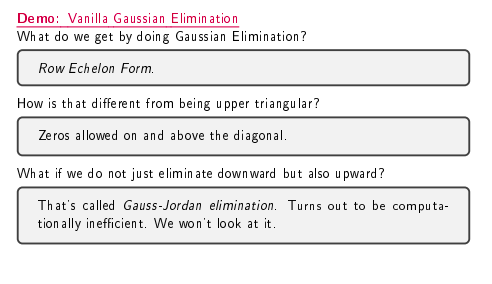
\includegraphics[width=\textwidth,height=\textheight,keepaspectratio]{lec6_rowE}
\end{center}

\begin{remark}
    Also note that a matrix is in row echelon form if the first non-zero entry of each row (what was the pivot during gaussian elimination) is to the first of the first non-zero entry of any preceding row; moreover, entries in rows above the pivot (but in the same column) must be $0$.
\end{remark}

\begin{center}
    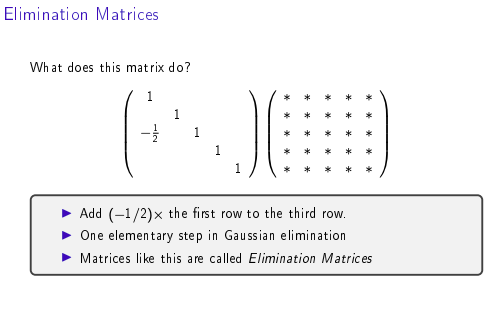
\includegraphics[width=\textwidth,height=\textheight,keepaspectratio]{lec6_elimM}
\end{center}

\begin{remark}
    If we add $k$ to the identity matrix at entry $i,j$, and left multiply the resultant
    matrix $C$ by some matrix of interest $A$, then the result is to take the $j$ th row of $A$
    multiply it by $k$ and then add it to $i$. We can undo this process by using the same
    matrix but, in place of $k$, using $-k$. This second matrix is the inverse to the elimination matrix $C$.
\end{remark}

\begin{center}
    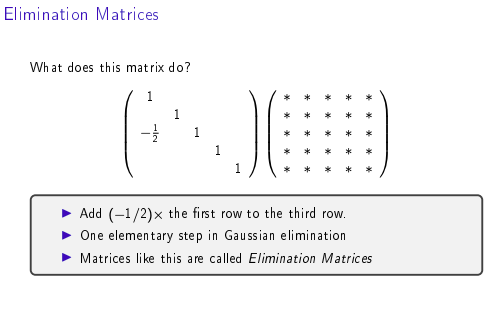
\includegraphics[width=\textwidth,height=\textheight,keepaspectratio]{lec6_elimM}
\end{center}


\begin{remark}
    Suppose that we multiply $A$ by an elimination matrix $M_1$, then by $M_2$ up to $M_l$,
    where $M_l$ is the last matrix required to turn $A$ into Row Echelon Form.
    Eventually, we will have 

    \[
        (M_l \dots M_1)A = U \implies A =  \inv{(M_l \dots M_1)}U
    \]

    At first glance, this is okay, because it turns out that left multiplication of an elimination matrix $X$ by $Y$ such that $X$ has a non-zero off diagonal at column $i$ and $Y$ has a non-zero off diagonal at column $j$ where $i < j$ results in an elimination matrix that just merges $X$ and $Y$ \footnote{Note that merging also takes place if we multiply two elimination matrices that have their off diagonal non-zero entry in the same column as each other.}

    For whatever reason, pivoting foils this attempt:

    \begin{center}
        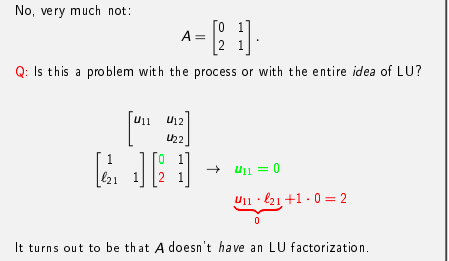
\includegraphics[width=\textwidth,height=\textheight,keepaspectratio]{lec6_pivotfail}
    \end{center}

    The solution is to repeatedly apply permutations to $A$ (in the form
    of permutation matrices) so that the pivot is the largest element
    in terms of absolute value in its column.

    Thus, we now have

    \[
        (M_lP_l \dots M_1P_1)A = U \implies A = \inv{(M_lP_l \dots M_1P_1)}U
    \]

    However, what should be $L$ above is not always left triangular. It can be shown that a factorization of $\inv{(M_lP_l \dots M_1P_1)}$ does, however, give us a lower triangular system.
\begin{center}
    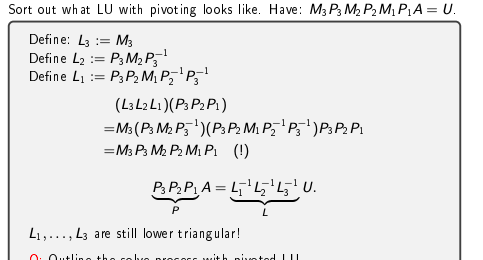
\includegraphics[width=\textwidth,height=\textheight,keepaspectratio]{lec6_pivotres}
\end{center}
\end{remark}

\begin{center}
    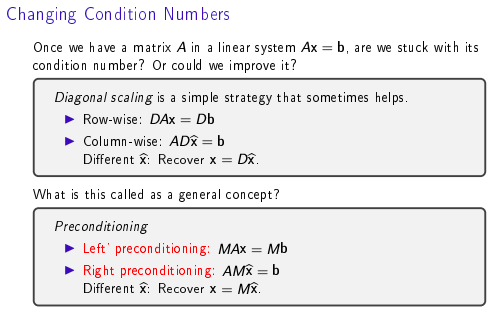
\includegraphics[width=\textwidth,height=\textheight,keepaspectratio]{lec6_precond}
\end{center}
\begin{remark}
    Suppose that $D$ above satisfies $k(D) \approx 1$. Then

    \[
        k(DA) = \norm{DA}\norm{\inv{(DA)}} \leq \norm{D}\norm{A}\norm{\inv{A}}\norm{\inv{D}} \leq k(A)
    \]

    so that the condition number of $K(DA)$ is no greater than the condition number of $A$.

    Assuming that $D$ is invertible, then the set of $x$ satisfying
    $Ax = b$ is precisely the set of $x$ satisfying $Ax = b$. Left multiplication
    by $D$ of $A$ is called, understandably, left preconditioning and scales
    $A$ in a row-wise manner; right multiplication by $D$ of $A$ is called right
    preconditioning.
\end{remark}


\begin{remark}
\begin{center}
    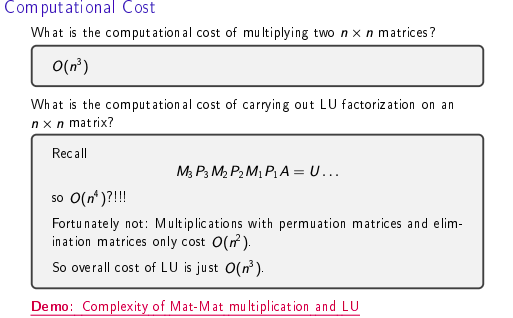
\includegraphics[width=\textwidth,height=\textheight,keepaspectratio]{lec6_compCost}
\end{center}

Multiplication by a permutation matrix is only an $n$ operation, since it involves switching rows. Multiplication by an elimination matrix simply involves scaling one row and mulitplying it by another, and this process is done at most $n$ times for any one elimination matrix (making it $O(n^2)$ as well). Since these transformations are applied at most $n$ times, the process of getting a matrix into $LU$ form is only $O(n^3)$.
\end{remark}

\begin{remark}

\begin{center}
    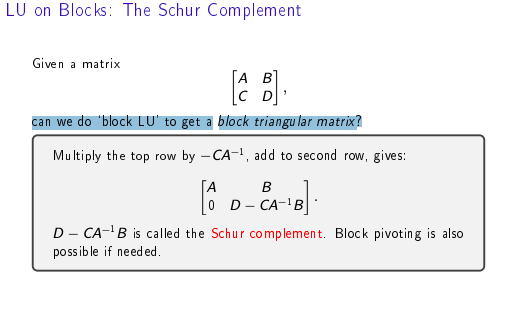
\includegraphics[width=\textwidth,height=\textheight,keepaspectratio]{lec6_luBlocks}
\end{center}

Not sure why this is significant.

\end{remark}


\begin{remark}
    Unresolved
\begin{center}
    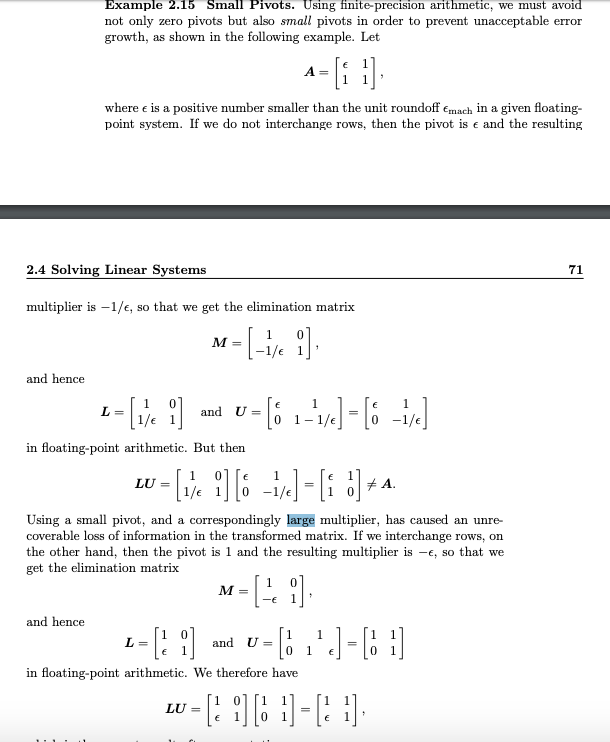
\includegraphics[width=\textwidth,height=\textheight,keepaspectratio]{lec6_smallPivotsBad}
\end{center}
\end{remark}

\begin{remark}
    Notice that if we already have an $LU$ factorization, then computing a rank $1$ update is just an $O(n^2)$ operation.
\begin{center}
    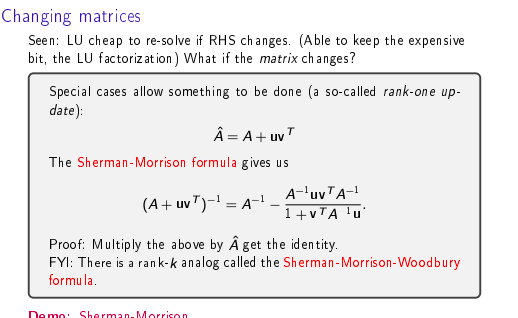
\includegraphics[width=\textwidth,height=\textheight,keepaspectratio]{lec6_shermanMorrison}
\end{center}

For 

\[
    \left( A + uv^T \right)^{-1}b = \inv{A}b - \frac{\left( \inv{A}u \right)v^T\inv{A}b}{1 + v^T\inv{A}u}
\]

And $\inv{A}x$ for any $x$ is an $O(n^2)$ operation. The only other operation in this formula is to compute a dot product.
\end{remark}

\begin{remark}
    \begin{center}
        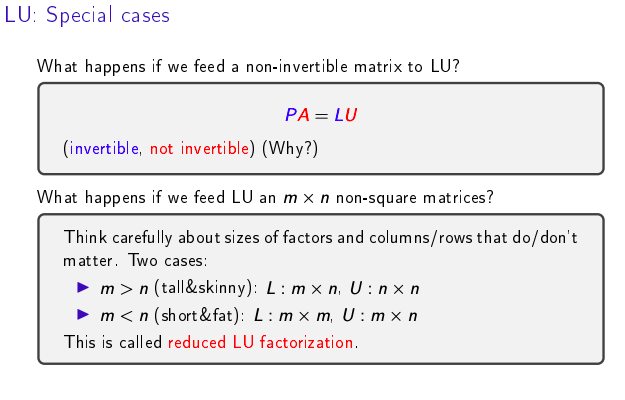
\includegraphics[width=\textwidth,height=\textheight,keepaspectratio]{lecture6_lu_special}
    \end{center}

    A matrix $A$ always admits an LU factorization, even if $A$
    is singular. First, observe that every column of $A$ must contain
    at least one non-zero number -- or else, why would the column
    be part of $A$. Thus, if a pivot entry does not contain a non-zero
    value, we can rotate rows so that the pivot entry does have
    a non-zero value. We then can apply elimination matrices, as needed,
    until all row values in the pivot's column are $0$. 

    The foregoing tells us that there still exists a sequence of
    permutations and elimination matrices that bring $A$ into upper
    triangular form. Since these matrices are each invertible, it follows that $L$ is still invertible. Since $\abs{PA} = 0$, we must have, therefore, $\abs{U} = 0$, which means that $0$ must occupy some diagonal entry of $U$.

    Why? A matrix fails to be invertible iff $0$ is an eigenvalue. $0$ is an eigenvalue iff some entry on the diagonal is $0$, because the eigenvalues of a triangular matrix are precisely its diagonal entries.

    Why are permutation matrices invertible? Group theory promises us that some power of a permutation brings it back to the identity. That is $P^k = I$ for some $I$. Thus $\inv{P} = P^{k-1}$.
\end{remark}

\begin{remark}
    Why can we take an $LU$ decomposition and then reduce it, as shown below?
    \begin{center}
        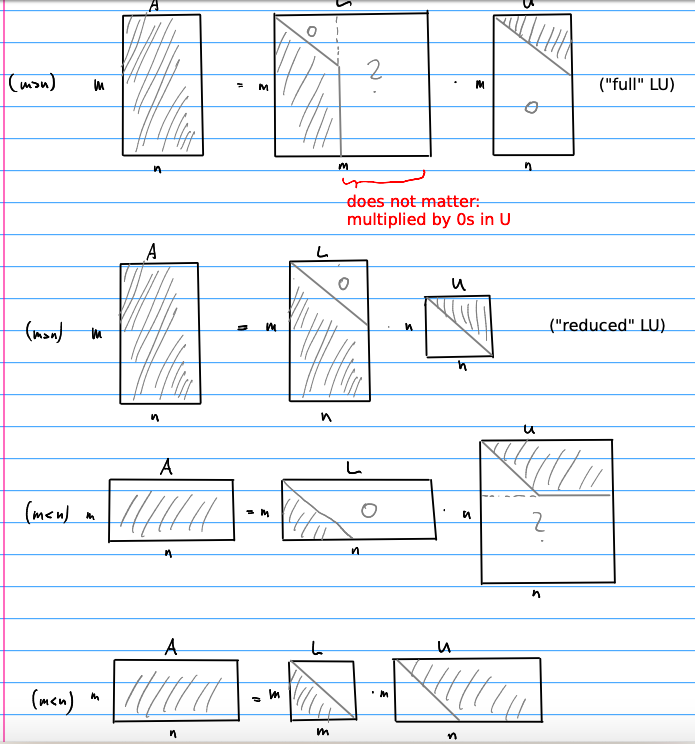
\includegraphics[width=\textwidth,height=\textheight,keepaspectratio]{lecture6_lu_reduced}
    \end{center}

    If $m > n$, applying elimination matrices that use row $n+1$ is a no-op, since the use of row $n$ has (along with prior use of rows $1 \dots n-1$) already made row $n+1$ be entirely $0$. or if $n > m$. As a consequence, in the unreduced LU factorization (the first and third pictures above), we see that every column in $\left\{ n+1 \dots m \right\}$ is really just $0$ except at a diagonal entry (where it is $1$). As the picture points out, however, determinining what exists in the unreduced $L$ is not useful, since $A = LU$ where $L = [Q B]$ and $U = \begin{bmatrix}
        Q' \\
        B' \\
    \end{bmatrix}$ where $Q = m \times n$, $B = m \times m-n$, $Q' = n \times n$ and $B' = m -n \times n$. Since $BB' = \mathbb{0}$, there is no need to store $B$ or $B'$.

    Using similar reasoning, we can understand the case that $n > m$.
\end{remark}

\section{Lecture 7}{Least Squares}
\begin{remark}
    We assume that we work with tall, skinny matrices that have full column rank.
\end{remark}
\begin{remark}
    \begin{center}
        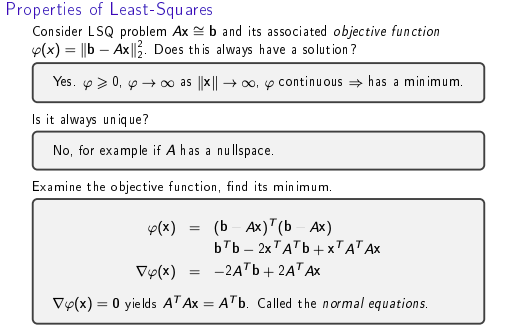
\includegraphics[width=\textwidth,height=\textheight,keepaspectratio]{lecture7_least_squares_prelim}
    \end{center}
    The textbook proves that there is always a unique vector $y \in \text{Span}(A)$ such that $\phi(y) = \norm{b - y}^2$ is minimal; as a consequence, there is at least one vector $x \in \R^m$ where $A$ is $\R^{n \times m}$ that minimizes $Ax \approx b$. This vector $x$ is unique iff $A$ is full rank.
\end{remark}

\begin{definition}
    A matrix $P$ is a projection if $P^2 = P$. A matrix is an orthogonal projection if $P^2 = P$ and $P^T = P$.
\end{definition}

\begin{proposition}
    If $P$ is an orthogonal projection, then the span of $P_{\perp} = (I - P)$ is orthogonal to the span of $P$.
\end{proposition}
\begin{proof}
    Given $x,y \in \R^n$, we see that

    \begin{align*}
        \inner{Px, (I - P)y} \\
        = \inner{Px, y - Py} \\
        = \inner{Px, y} - \inner{Px, Py} \\
        = \inner{Px, y} - \inner{x, Py} \\
        = 0
    \end{align*}
\end{proof}

\begin{corollary}
    Given an orthogonal projection $P$, any vector $x$ can be expressed as $x = Px + P_{\perp}x$.
\end{corollary}

\begin{proposition}
    The vector $x$ satisfying $\min_{x \in \R^n} \norm{Ax - b}_2$ is precisely the $x$ such that $Ax = Pb$ where $P$ is a projection onto $A$.
\end{proposition}

\begin{proof}
    Note that in what follows, all norms refer to the $2$ norm.
    \begin{align*}
        \norm{Ax - b} = \norm{P(Ax -b) + P_{\perp}(Ax - b)} \\
        \intertext{Since $P$ and $P_{\perp}$ map to orthogonal subspaces, we can apply the Pythagorean theorem} \\
        = \norm{P(Ax -b)} + \norm{P_{\perp}(Ax - b)} \\
        = \norm{P(Ax -b)} + \norm{-P_{\perp}b} \\
        = \norm{P(Ax -b)} + \norm{P_{\perp}b} \\
        = \norm{(Ax - Pb)} + \norm{P_{\perp}b} \\
        \intertext{The RHS is fixed, so we can only minimize the LHS} \\
    \end{align*}
\end{proof}

\begin{corollary}
    The $x$ aforementioned is $\inv{(A^TA)}A^Tb$ 
\end{corollary}
\begin{proof}
    \begin{align*}
        Ax = Pb \\
        \iff A^TAx = A^TPb \\
        \iff A^TAx = (PA)^Tb \\
        \iff A^TAx = (A)^Tb \\
        \iff x = \inv{(A^TA)}(A)^Tb \\
    \end{align*}
\end{proof}

\begin{proposition}
    $P = \inv{(A^TA)}A^T$ is an orthogonal projection, assuming
    that $A$ has full column rank.
\end{proposition}
\begin{proof}
    Verify to yourself that it is symmetric and $P^2 = P$. Also verify that $\text{span}(P) = \text{span}(A)$.
\end{proof}

\begin{corollary}
    The $x$ aformentioned is orthogonal to $b- Ax$, the residual.
\end{corollary}

\begin{proof}
    \begin{align*}
        b = Pb + P_{\perp}b \\
        \intertext{Substitute the definition of $x$ and $P$ found above}  \\
        b = Ax + (b - Ax) \\
    \end{align*}
\end{proof}

\begin{proposition}
    Suppose we know that the columns of $Q \in \R^{m \times n}$ form an orthonormal basis for $\text{span}(A)$. Then $QQ^T$ is an orthogonal projector for $A$.
\end{proposition}
\begin{proof}
    $(QQ^T)(QQ^T) = QQ^T$. Thus, this matrix is a projection; is it also clearly symmetric; finally, note that its span is precisely the span of $A$.
\end{proof}

\begin{corollary}
    With $Q$ as above and $P = QQ^T$, then the optimal $x$ satisfying $Ax \approx b$ is $Ax = Pb$. Leftmulitply both sides by $Q^T$ to obtain

    \[
        Q^TAx = Q^Tb
    \]

    If we do this, we can avoid the hassle of using the normal equations.
\end{corollary}

\begin{definition}
    I take the following as definitions. No time to look into their proofs:
    \begin{center}
        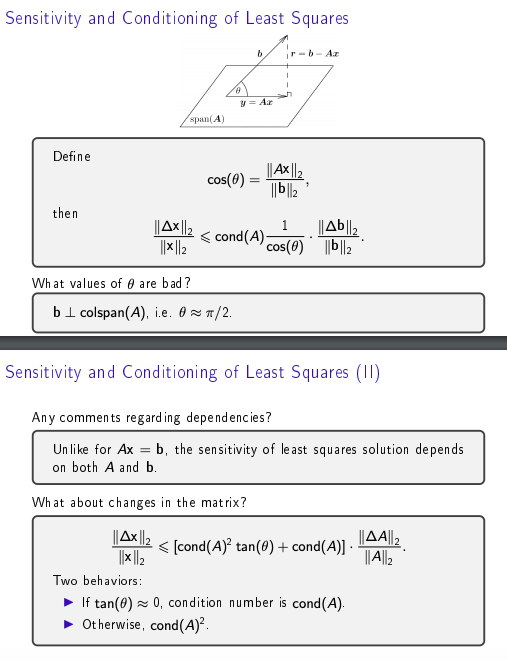
\includegraphics[width=\textwidth,height=\textheight,keepaspectratio]{lecture7_least_squares_cond}
    \end{center}
\end{definition}

\end{document}






\section{Lecture 7}

\subsection{Quiz}




